% fsb: how it is built. Beamer slides; build with "make" in this folder.
\documentclass[aspectratio=169,11pt]{beamer}
\usetheme{moloch}
\usepackage{tikz}
\usetikzlibrary{arrows.meta,positioning,fit,backgrounds,calc}
\usepackage{booktabs}

\title{fsb}
\subtitle{A read-only file browser in your web browser, and how it is built}
\date{October 2026 \textperiodcentered{} describes fsb 1.0.12}

\definecolor{guard}{HTML}{B5432C}
\definecolor{net}{HTML}{2C6CB5}
\definecolor{ui}{HTML}{3A8A4F}
\tikzset{
  box/.style={draw, rounded corners=2pt, align=center, minimum height=8mm,
    inner sep=4pt, font=\small},
  stage/.style={box, minimum width=34mm, font=\footnotesize},
  no/.style={font=\scriptsize, text=guard},
  flow/.style={-{Latex[length=2mm]}, thick},
}
\newcommand{\code}[1]{\texttt{\small #1}}

\begin{document}

\maketitle

\begin{frame}{What fsb is}
  \begin{itemize}
    \item One Go binary that serves a browser UI on \code{127.0.0.1}
    \item Browse, sort, filter, search and preview your own files, on macOS or Linux
    \item \textbf{Read-only by construction}: only \code{GET} endpoints, no code
      that writes your files
    \item \textbf{Local-only}: loopback address, Host and Origin checks,
      a single-use launch token
    \item \textbf{Deny rules} (\code{\textasciitilde/.ssh}, keychains, browser
      profiles, \ldots) refused on every path, answered as ``not found''
  \end{itemize}
  \vfill
  \small The promise is that it is safe to point at a real filesystem.
  Most of the code exists to keep that promise.
\end{frame}

\begin{frame}{Architecture}
  \centering
  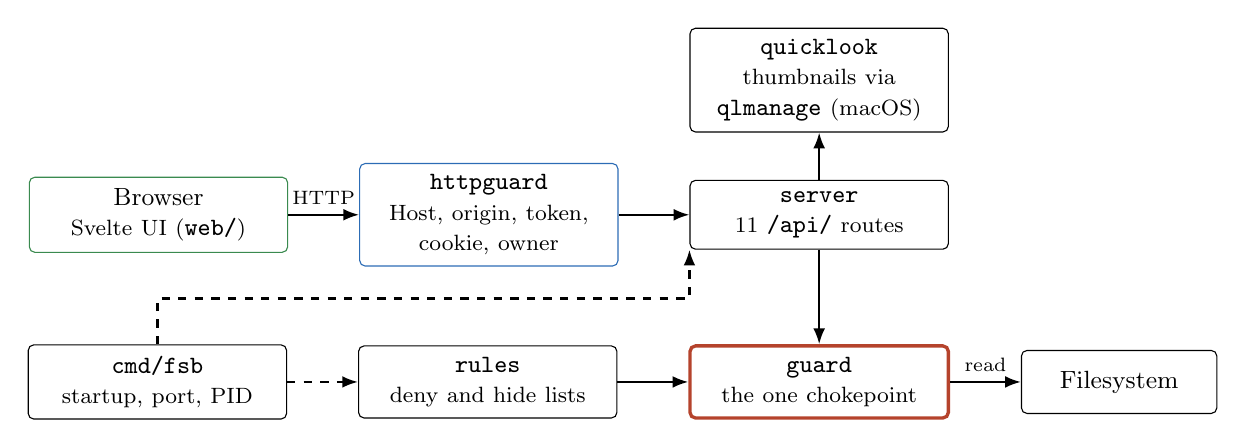
\begin{tikzpicture}[node distance=6mm and 9mm]
    \node[box, draw=ui, text width=30mm] (ui) {Browser\\\footnotesize Svelte UI (\code{web/})};
    \node[box, draw=net, right=of ui, text width=30mm] (mw) {\code{httpguard}\\\footnotesize Host, origin, token, cookie, owner};
    \node[box, right=of mw, text width=30mm] (srv) {\code{server}\\\footnotesize 11 \code{/api/} routes};
    \node[box, draw=guard, very thick, below=12mm of srv, text width=30mm] (g) {\code{guard}\\\footnotesize the one chokepoint};
    \node[box, left=of g, text width=30mm] (rules) {\code{rules}\\\footnotesize deny and hide lists};
    \node[box, right=of g, text width=22mm] (fs) {Filesystem};
    \node[box, above=of srv, text width=30mm] (ql) {\code{quicklook}\\\footnotesize thumbnails via \code{qlmanage} (macOS)};
    \node[box, left=of rules, text width=30mm] (main) {\code{cmd/fsb}\\\footnotesize startup, port, PID};

    \draw[flow] (ui) -- node[above, font=\scriptsize]{HTTP} (mw);
    \draw[flow] (mw) -- (srv);
    \draw[flow] (srv) -- (g);
    \draw[flow] (srv) -- (ql);
    \draw[flow] (rules) -- (g);
    \draw[flow] (g) -- node[above, font=\scriptsize]{read} (fs);
    \draw[flow, dashed] (main) -- (rules);
    \draw[flow, dashed] (main.north) |- ($(ui.south)!.5!(main.north)$) -| (srv.south west);
  \end{tikzpicture}
  \vfill
  \small Every file access goes through \code{guard}; no handler opens a path itself.
\end{frame}

\begin{frame}{Startup: \code{cmd/fsb} \code{run()}}
  \centering
  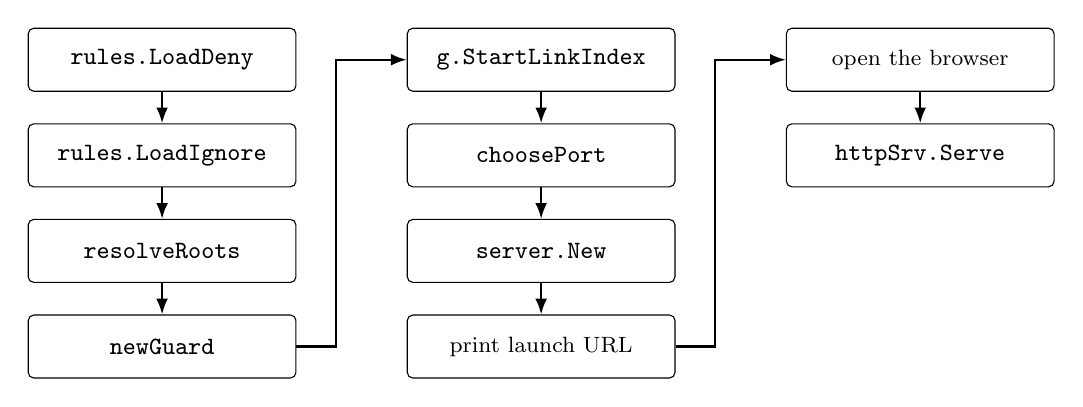
\begin{tikzpicture}[node distance=4mm and 6mm, every node/.style={stage}]
    \node (a) {\code{rules.LoadDeny}};
    \node[below=of a] (b) {\code{rules.LoadIgnore}};
    \node[below=of b] (c) {\code{resolveRoots}};
    \node[below=of c] (d) {\code{newGuard}};
    \node[right=14mm of a] (e) {\code{g.StartLinkIndex}};
    \node[below=of e] (f) {\code{choosePort}};
    \node[below=of f] (g) {\code{server.New}};
    \node[below=of g] (h) {print launch URL};
    \node[right=14mm of e] (i) {open the browser};
    \node[below=of i] (j) {\code{httpSrv.Serve}};
    \draw[flow] (a) -- (b); \draw[flow] (b) -- (c); \draw[flow] (c) -- (d);
    \draw[flow] (d.east) -- ++(5mm,0) |- (e.west);
    \draw[flow] (e) -- (f); \draw[flow] (f) -- (g); \draw[flow] (g) -- (h);
    \draw[flow] (h.east) -- ++(5mm,0) |- (i.west);
    \draw[flow] (i) -- (j);
  \end{tikzpicture}
  \vfill
  \begin{itemize}\small
    \item Core deny rules are built in; a missing one raises a warning banner
    \item The hard-link index builds in the background; until it is ready,
      files with several names are refused
    \item The port is on \code{127.0.0.1} only; the interface cannot be configured
  \end{itemize}
\end{frame}

\begin{frame}{One request: \code{GET /\emph{prefix}/api/file?path=\ldots}}
  \centering
  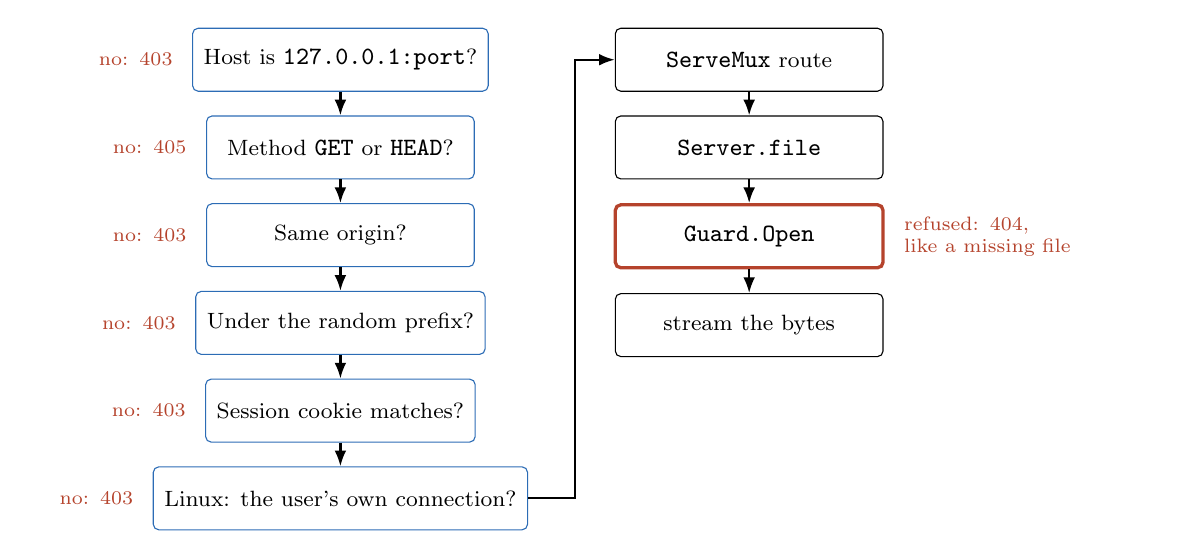
\begin{tikzpicture}[node distance=3mm and 8mm, every node/.style={stage}]
    \node[draw=net] (h) {Host is \code{127.0.0.1:port}?};
    \node[draw=net, below=of h] (m) {Method \code{GET} or \code{HEAD}?};
    \node[draw=net, below=of m] (o) {Same origin?};
    \node[draw=net, below=of o] (p) {Under the random prefix?};
    \node[draw=net, below=of p] (c) {Session cookie matches?};
    \node[draw=net, below=of c] (u) {Linux: the user's own connection?};
    \node[right=16mm of h] (r) {\code{ServeMux} route};
    \node[below=of r] (s) {\code{Server.file}};
    \node[draw=guard, very thick, below=of s] (g) {\code{Guard.Open}};
    \node[below=of g] (w) {stream the bytes};
    \foreach \x/\y in {h/m, m/o, o/p, p/c, c/u, r/s, s/g, g/w} \draw[flow] (\x) -- (\y);
    \draw[flow] (u.east) -- ++(6mm,0) |- (r.west);
    \foreach \x in {h,o,p,c,u} \node[no, anchor=east, draw=none, minimum width=0pt, text width=12mm, align=right] at ($(\x.west)+(-1mm,0)$) {no: 403};
    \node[no, anchor=east, draw=none, minimum width=0pt, text width=12mm, align=right] at ($(m.west)+(-1mm,0)$) {no: 405};
    \node[no, anchor=west, draw=none, minimum width=0pt, text width=30mm, align=left] at ($(g.east)+(1mm,0)$) {refused: 404,\\like a missing file};
  \end{tikzpicture}
  \vfill
  \small Left column: \code{httpguard.Middleware}, the same for every route.
  On Linux the owner of the connection is looked up once per connection;
  macOS has no such check.
\end{frame}

\begin{frame}{The chokepoint: \code{guard.open}}
  \centering
  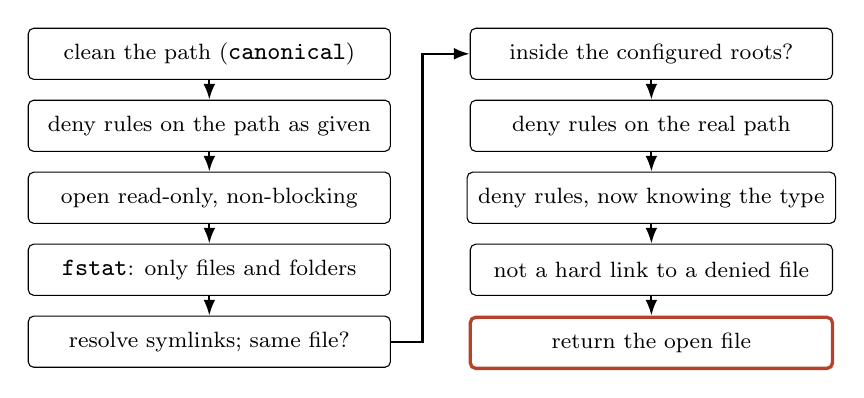
\begin{tikzpicture}[node distance=2.5mm and 10mm, every node/.style={stage, minimum width=46mm, minimum height=6.5mm}]
    \node (1) {clean the path (\code{canonical})};
    \node[below=of 1] (2) {deny rules on the path as given};
    \node[below=of 2] (3) {open read-only, non-blocking};
    \node[below=of 3] (4) {\code{fstat}: only files and folders};
    \node[below=of 4] (5) {resolve symlinks; same file?};
    \node[right=of 1] (6) {inside the configured roots?};
    \node[below=of 6] (7) {deny rules on the real path};
    \node[below=of 7] (8) {deny rules, now knowing the type};
    \node[below=of 8] (9) {not a hard link to a denied file};
    \node[draw=guard, very thick, below=of 9] (10) {return the open file};
    \foreach \x/\y in {1/2, 2/3, 3/4, 4/5, 6/7, 7/8, 8/9, 9/10} \draw[flow] (\x) -- (\y);
    \draw[flow] (5.east) -- ++(4mm,0) |- (6.west);
  \end{tikzpicture}
  \vfill
  \begin{itemize}\small
    \item Opening first and then checking what was opened closes the race
      between check and use
    \item FIFOs, sockets and devices are rejected before anything is read
  \end{itemize}
\end{frame}

\begin{frame}{Logging in without a password}
  \centering
  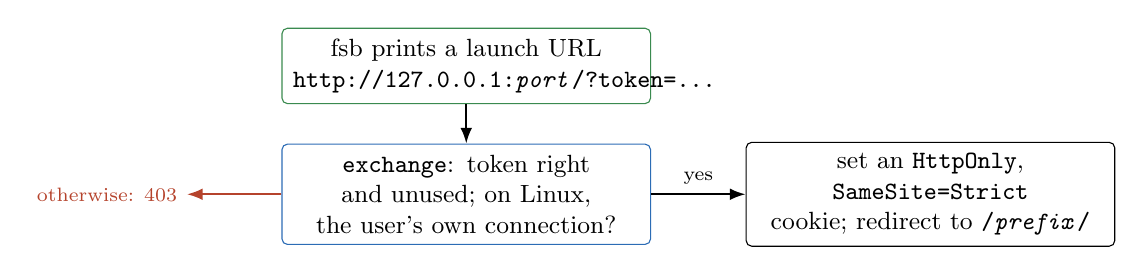
\begin{tikzpicture}[node distance=5mm and 12mm]
    \node[box, draw=ui, text width=44mm] (t) {fsb prints a launch URL\\\scriptsize\code{http://127.0.0.1:\emph{port}/?token=\ldots}};
    \node[box, draw=net, below=of t, text width=44mm] (x) {\code{exchange}: token right\\and unused; on Linux,\\the user's own connection?};
    \node[box, right=of x, text width=44mm] (k) {set an \code{HttpOnly}, \code{SameSite=Strict}\\cookie; redirect to \code{/\emph{prefix}/}};
    \node[no, left=of x] (n) {otherwise: 403};
    \draw[flow] (t) -- (x); \draw[flow] (x) -- node[above, font=\scriptsize]{yes} (k);
    \draw[flow, guard] (x) -- (n);
  \end{tikzpicture}
  \vfill
  \begin{itemize}\small
    \item The token works once (an atomic compare-and-swap), then leaves the address bar
    \item The prefix is random and not in the launch URL: a user who reads the
      opener's command line learns only a spent token
    \item Other paths are refused like unauthenticated requests; comparisons are constant-time
    \item Linux: another user's connection is refused, at launch and on every
      request, without using up the token
  \end{itemize}
\end{frame}

\begin{frame}[plain]
  \centering
  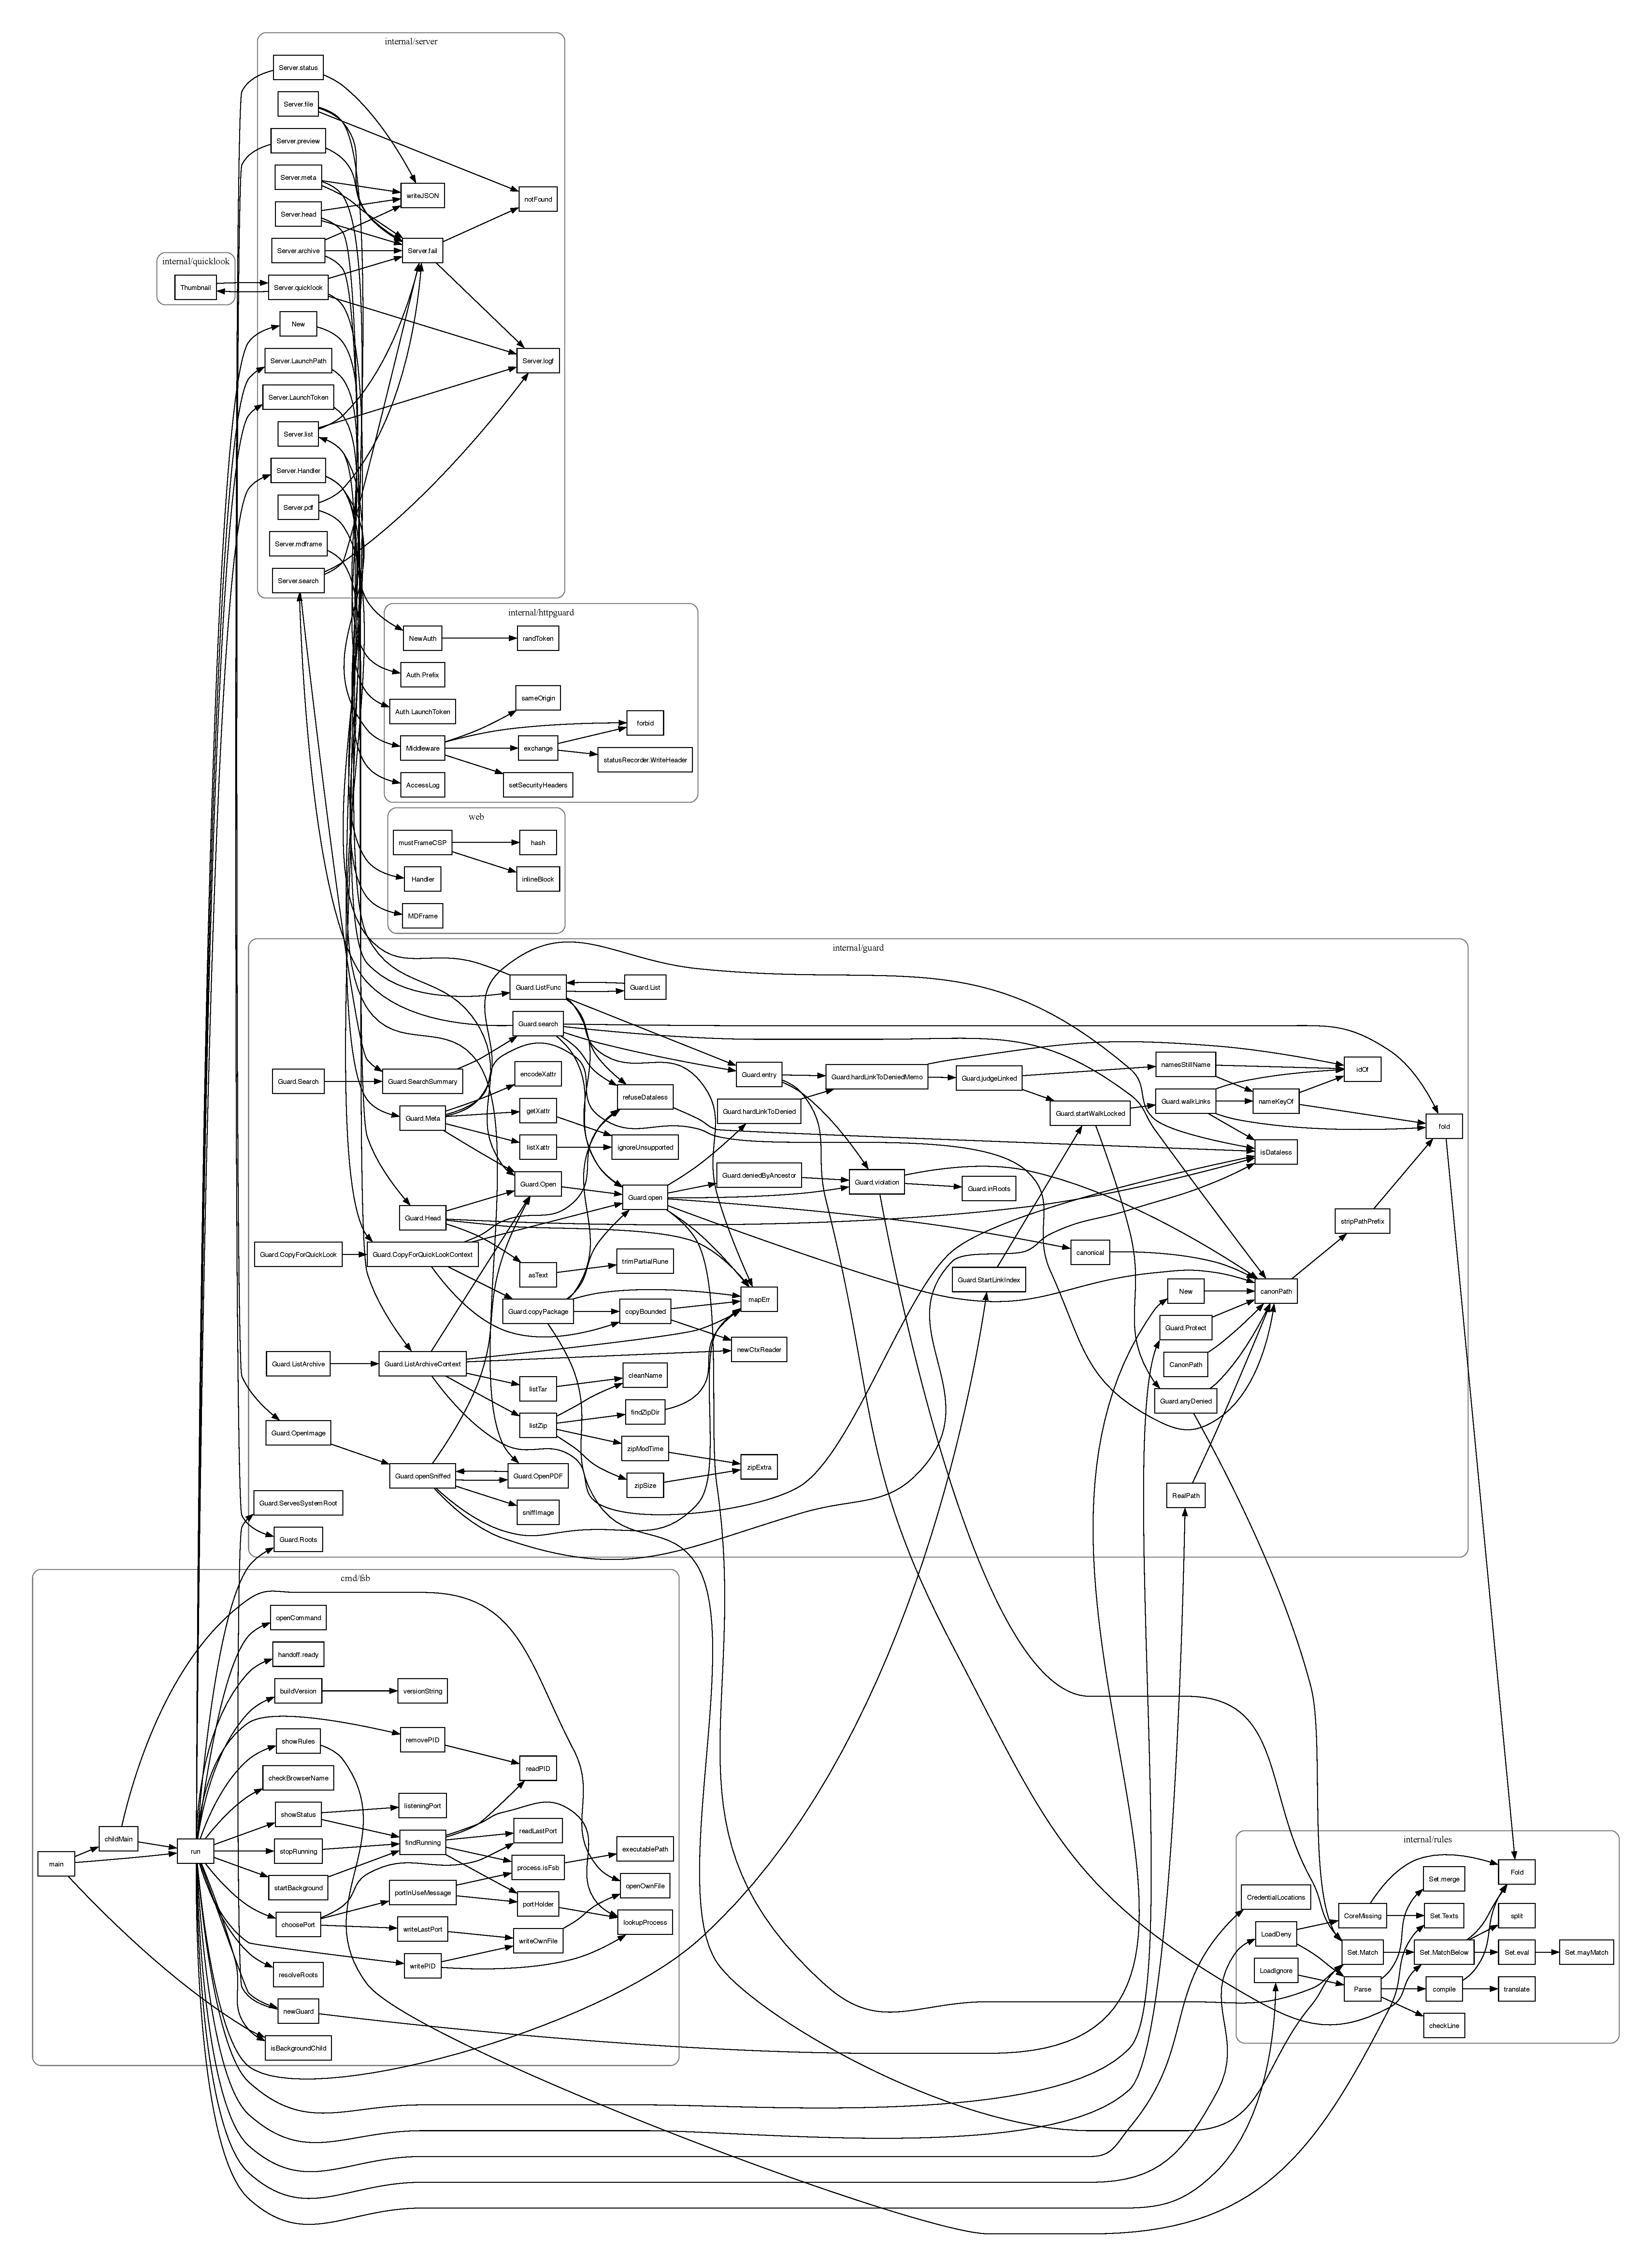
\includegraphics[height=0.93\textheight]{callgraph.pdf}\\[-1mm]
  {\scriptsize Every call between fsb's own functions: 162 functions, 251 calls.
  Generated from the code, not drawn.}
\end{frame}

\begin{frame}{Calls between packages}
  \centering
  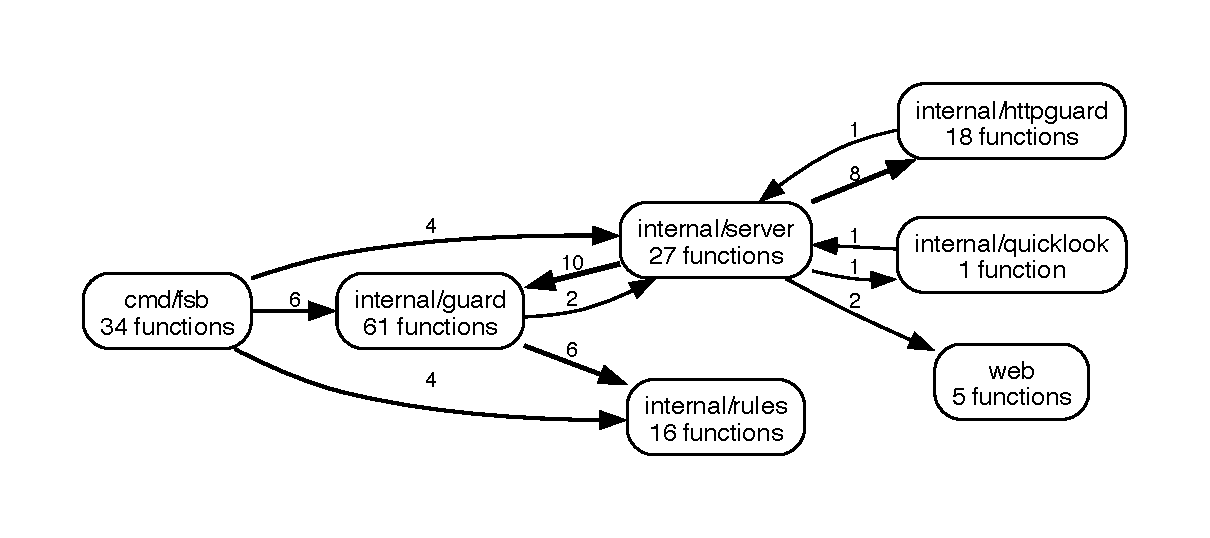
\includegraphics[width=\textwidth,height=0.62\textheight,keepaspectratio]{packages.pdf}
  \vfill
  \small The same graph folded by package; numbers are distinct caller--callee pairs.
  The arrows back into \code{server} are callbacks: \code{server} hands
  \code{guard} and \code{quicklook} a function to call for each result.
\end{frame}

\begin{frame}{Where the functions are}
  \centering
  \begin{tabular}{lrl}
    \toprule
    Package & Functions & Role \\
    \midrule
    \code{internal/guard}     & 61 & the chokepoint: open, list, search, archives, links \\
    \code{cmd/fsb}            & 34 & startup, port choice, background mode, opener \\
    \code{internal/server}    & 27 & HTTP handlers \\
    \code{internal/rules}     & 16 & gitignore-style rule matching \\
    \code{internal/httpguard} & 18 & localhost protections, login, connection owner \\
    \code{web}                &  5 & embedded UI, Markdown frame \\
    \code{internal/quicklook} &  1 & thumbnails for Office and iWork \\
    \bottomrule
  \end{tabular}
  \vfill
  \small Counted from the call graph: functions that call or are called by
  another fsb function.
\end{frame}

\begin{frame}{By the numbers}
  \begin{columns}[T]
    \column{0.48\textwidth}
    \begin{itemize}
      \item About 4,000 lines of Go
      \item About 8,100 lines of Go tests
      \item About 3,100 lines of Svelte and TypeScript
      \item Browser tests in Chrome and Safari, against macOS and four
        Linux distributions
    \end{itemize}
    \column{0.48\textwidth}
    \begin{itemize}
      \item About 140 commits since 20 September 2026
      \item Functional, design and algebraic specs in \LaTeX
      \item Independent reviews at each new boundary
      \item Source only; provided as-is
    \end{itemize}
  \end{columns}
\end{frame}

\begin{frame}[fragile]{How these slides were made}
  \begin{enumerate}
    \item \textbf{Call graph} from Go's own analysis (\code{golang.org/x/tools}):
\begin{verbatim}
callgraph -algo=vta ./cmd/fsb
\end{verbatim}
    \item \textbf{Filter}: a short Python script keeps calls between fsb's own
      functions and writes a Graphviz file; \code{dot} draws it
    \item \textbf{Diagrams}: drawn by hand in Ti\emph{k}Z, checked against the graph
    \item \textbf{Slides}: \LaTeX{} Beamer, theme \emph{moloch}
  \end{enumerate}
  \vfill
  \small \code{make} in \code{docs/talk/} rebuilds everything from the current code.
\end{frame}

\end{document}
